%----------------------------------------------------------------------------------------
%	PACKAGES AND OTHER DOCUMENT CONFIGURATIONS
%----------------------------------------------------------------------------------------

\documentclass{article}

\usepackage{fancyhdr} % Required for custom headers
\usepackage{lastpage} % Required to determine the last page for the footer
\usepackage{extramarks} % Required for headers and footers
\usepackage[usenames,dvipsnames]{color} % Required for custom colors
\usepackage{pgf} % Required to insert pgf plots from matplotlib
\usepackage{graphicx} % Required to insert images
\usepackage{listings} % Required for insertion of code
\usepackage{courier} % Required for the courier font
\usepackage{lipsum} % Used for inserting dummy 'Lorem ipsum' text into the template
\usepackage[utf8]{inputenc}
\usepackage[ngerman]{babel}
\usepackage{subcaption, caption, tabularx, minted}
\usepackage{hyperref}

% Margins
\topmargin=-0.45in
\evensidemargin=0in
\oddsidemargin=0in
\textwidth=6.5in
\textheight=9.0in
\headsep=0.25in

\linespread{1.1} % Line spacing

% Set up the header and footer
\pagestyle{fancy}
%\lhead{\hmwkAuthorName} % Top left header
\chead{\hmwkClass\ : \hmwkTitle} % Top center head
\rhead{\firstxmark} % Top right header
\lfoot{\lastxmark} % Bottom left footer
\cfoot{} % Bottom center footer
\rfoot{Page\ \thepage\ of\ \protect\pageref{LastPage}} % Bottom right footer
\renewcommand\headrulewidth{0.4pt} % Size of the header rule
\renewcommand\footrulewidth{0.4pt} % Size of the footer rule

\setlength\parindent{0pt} % Removes all indentation from paragraphs

%----------------------------------------------------------------------------------------
%	CODE INCLUSION CONFIGURATION
%----------------------------------------------------------------------------------------

\definecolor{MyDarkGreen}{rgb}{0.0,0.4,0.0} % This is the color used for comments
\lstloadlanguages{Perl} % Load Perl syntax for listings, for a list of other languages supported see: ftp://ftp.tex.ac.uk/tex-archive/macros/latex/contrib/listings/listings.pdf
\lstset{language=Perl, % Use Perl in this example
        frame=single, % Single frame around code
        basicstyle=\small\ttfamily, % Use small true type font
        keywordstyle=[1]\color{Blue}\bf, % Perl functions bold and blue
        keywordstyle=[2]\color{Purple}, % Perl function arguments purple
        keywordstyle=[3]\color{Blue}\underbar, % Custom functions underlined and blue
        identifierstyle=, % Nothing special about identifiers                                         
        commentstyle=\usefont{T1}{pcr}{m}{sl}\color{MyDarkGreen}\small, % Comments small dark green courier font
        stringstyle=\color{Purple}, % Strings are purple
        showstringspaces=false, % Don't put marks in string spaces
        tabsize=5, % 5 spaces per tab
        %
        % Put standard Perl functions not included in the default language here
        morekeywords={rand},
        %
        % Put Perl function parameters here
        morekeywords=[2]{on, off, interp},
        %
        % Put user defined functions here
        morekeywords=[3]{test},
       	%
        morecomment=[l][\color{Blue}]{...}, % Line continuation (...) like blue comment
        numbers=left, % Line numbers on left
        firstnumber=1, % Line numbers start with line 1
        numberstyle=\tiny\color{Blue}, % Line numbers are blue and small
        stepnumber=5 % Line numbers go in steps of 5
}

% Creates a new command to include a perl script, the first parameter is the filename of the script (without .pl), the second parameter is the caption
\newcommand{\perlscript}[2]{
\begin{itemize}
\item[]\lstinputlisting[caption=#2,label=#1]{#1.pl}
\end{itemize}
}

%----------------------------------------------------------------------------------------
%	DOCUMENT STRUCTURE COMMANDS
%	Skip this unless you know what you're doing
%----------------------------------------------------------------------------------------

% Header and footer for when a page split occurs within a problem environment
\newcommand{\enterProblemHeader}[1]{
%\nobreak\extramarks{#1}{#1 continued on next page\ldots}\nobreak
%\nobreak\extramarks{#1 (continued)}{#1 continued on next page\ldots}\nobreak
}

% Header and footer for when a page split occurs between problem environments
\newcommand{\exitProblemHeader}[1]{
%\nobreak\extramarks{#1 (continued)}{#1 continued on next page\ldots}\nobreak
%\nobreak\extramarks{#1}{}\nobreak
}

\setcounter{secnumdepth}{0} % Removes default section numbers
\newcounter{homeworkProblemCounter} % Creates a counter to keep track of the number of problems

\newcommand{\homeworkProblemName}{}
\newenvironment{homeworkProblem}[1][Problem \arabic{homeworkProblemCounter}]{ % Makes a new environment called homeworkProblem which takes 1 argument (custom name) but the default is "Problem #"
\stepcounter{homeworkProblemCounter} % Increase counter for number of problems
\renewcommand{\homeworkProblemName}{#1} % Assign \homeworkProblemName the name of the problem
\section{\homeworkProblemName} % Make a section in the document with the custom problem count
%\enterProblemHeader{\homeworkProblemName} % Header and footer within the environment
}{
%\exitProblemHeader{\homeworkProblemName} % Header and footer after the environment
}

\newcommand{\problemAnswer}[1]{ % Defines the problem answer command with the content as the only argument
\noindent\framebox[\columnwidth][c]{\begin{minipage}{0.98\columnwidth}#1\end{minipage}} % Makes the box around the problem answer and puts the content inside
}

\newcommand{\homeworkSectionName}{}
\newenvironment{homeworkSection}[1]{ % New environment for sections within homework problems, takes 1 argument - the name of the section
\renewcommand{\homeworkSectionName}{#1} % Assign \homeworkSectionName to the name of the section from the environment argument
\subsection{\homeworkSectionName} % Make a subsection with the custom name of the subsection
%\enterProblemHeader{\homeworkProblemName\ [\homeworkSectionName]} % Header and footer within the environment
}{
%\enterProblemHeader{\homeworkProblemName} % Header and footer after the environment
}

%----------------------------------------------------------------------------------------
%	NAME AND CLASS SECTION
%----------------------------------------------------------------------------------------

\newcommand{\hmwkTitle}{Exercise\ \#3} % Assignment title
\newcommand{\hmwkDueDate}{Tuesday,\ May 12,\ 2015} % Due date
\newcommand{\hmwkClass}{Advanced Parallel Computing} % Course/class
\newcommand{\hmwkClassTime}{} % Class/lecture time
\newcommand{\hmwkClassInstructor}{} % Teacher/lecturer
\newcommand{\hmwkAuthorName}{Svend Dorkenwald, Günther Schindler} % Your name

%----------------------------------------------------------------------------------------
%	TITLE PAGE
%----------------------------------------------------------------------------------------

\title{
\vspace{2in}
\textmd{\textbf{\hmwkClass:\ \hmwkTitle}}\\
\normalsize\vspace{0.1in}\small{Due\ on\ \hmwkDueDate}\\
\vspace{0.1in}\large{\textit{\hmwkClassTime}}
\vspace{3in}
}

\author{\textbf{\hmwkAuthorName}}
\date{} % Insert date here if you want it to appear below your name

%----------------------------------------------------------------------------------------

\begin{document}

\maketitle

%----------------------------------------------------------------------------------------
%	TABLE OF CONTENTS
%----------------------------------------------------------------------------------------

%\setcounter{tocdepth}{1} % Uncomment this line if you don't want subsections listed in the ToC

\newpage
\tableofcontents
\newpage

%----------------------------------------------------------------------------------------
%	Reading
%----------------------------------------------------------------------------------------

\begin{homeworkProblem}[Reading]

\subsection{Cost-Effective Parallel Computing}
The authors David A. Wood and Mark D. Hill show in their paper 'Cost-Effective Parallel 
Computing' that parallel systems can be cost-effective at modest speedups when memory cost
is significant fraction of system cost. They want to disprove the claim that parallel 
computing is only worthwile when applications achieve nearly linear speedup. To do that the 
researcher introduce the costup factor - the parallel system cost divided by uniprocessor
cost - and compare it to the classical speedup.
\\
Their results show that parallel computing can cost-effective maximize throughput whenever
speedup exceeds costup. Furthermore they expose when memory is sufficiently large, more 
than one processor may be needed to efficiently utilize the memory.
\\
In our opinion the reasoning of the authors is correct although their results are not 
groundbreaking. However, they results are solid arguments to disprove Amdahl's Law 
once again. Thus, we weakly accept this paper.
\subsection{A Survey of Cache Coherence Schemes for Multiprocessor}

\end{homeworkProblem}

%----------------------------------------------------------------------------------------
%	Shared Counter
%----------------------------------------------------------------------------------------

\begin{homeworkProblem}[Shared Counter]
As part of this exercise we should implement a Pthread program which results in a counter.
A mutex has to be used to ensure mutual exclustion when incrementing the counter.
\\
The following listening gives the algorithm which we implemented for this.
\begin{lstlisting}{c}
void vCountMutex(void *arg){
  int i, iID;
  iID = (intptr_t) arg;
  /* Synchronize threads */
  pthread_barrier_wait(&barrier);
  /* Start incrementation process */
  for(i = (iID*iC)/iN; i < ((iID+1)*iC)/iN; i++){
    /* Lock mutex */
    pthread_mutex_lock(&mutex);
    /* Increment count variable */
    vInc(&iCount);
    /* Unlock mutex */
    pthread_mutex_unlock(&mutex);
  }
}
\end{lstlisting}
Depending on the thread-ID (arg) every thread increments the count variable until the variable
reaches the C value. If we count without the mutual exclusion, data races result in a 
mismatch between the counter variable and the C value. 
\end{homeworkProblem}

%----------------------------------------------------------------------------------------
%	Shared counter revisited
%----------------------------------------------------------------------------------------

\begin{homeworkProblem}[Shared Counter Revisited]
Next, we should implement two alternative counter update methods. First, we use the atomic
operation \_\_sync\_add\_and\_fetch().
\begin{lstlisting}{c}
void vCountAtom(void *arg){
  int i, iID;
  iID = (intptr_t) arg;
  /* Synchronize threads */
  pthread_barrier_wait(&barrier);
  /* Start incrementation process */
  for(i = (iID*iC)/iN; i < ((iID+1)*iC)/iN; i++){
    /* Increment count variable */
    __sync_add_and_fetch(&iCount,1);
  }
}
\end{lstlisting}
As we can see, with the atomic operation there is no need for locking like the PThread
mutex anymore. This is because the fetch-and-add instruction allows any processor to 
automatically increment a value in memory, preventing multiple processor collisions.
\\\\
Based on this operation we also implemented our own locking mechanism as followed:
\begin{lstlisting}{c}
typedef struct {
  int ticket;
  int users;
} lock_t;

static void lock_rmw(lock_t *t){
  int me = __sync_add_and_fetch(&(t->users), 1);
  while (t->ticket != me)
    cpu_relax();
}

static void unlock_rmw(lock_t *t){
  __sync_add_and_fetch(&(t->ticket), 1);
}
\end{lstlisting}
In this case we need a atomic operation because this CPU instruction automatically modifies
the contents of a memory location instead of the cached value.
\end{homeworkProblem}
\pagebreak
%----------------------------------------------------------------------------------------
%	Shared counter performance analysis
%----------------------------------------------------------------------------------------

\begin{homeworkProblem}[Shared counter performance analysis]
As part of this exercise we should perform a performance analysis of the three 
different shared counter implementations. 
Following table shows the results of this performance analysis. Time is given in us and the 
update-rate is given in $10^9$/s.
\\
\begin{tabular}{|c|c|c|c|c|c|c|}\hline
   Thread \\Count & Time[Mutex] & Updates[Mutex] & Time[Atomic] & Updates[Atomic] & Time[RMW] & Updates[RMW] \\ \hline
   1 & 147 & 1.36 & 48 & 4.15 & 89 & 2.24  \\ \hline
   2 & 314 & 0.64 & 82 & 2.43 & 1260 & 0.16  \\ \hline
   4 & 1114 & 0.18 & 174 & 1.15 & 1494 & 0.13  \\ \hline
   8 & 318 & 0.63 & 180 & 1.11 & 2706 & 0.07  \\ \hline
   12 & 357 & 0.56 & 222 & 0.9 & 3781 & 0.05  \\ \hline
   16 & 315 & 0.63 & 187 & 1.07 & 5051 & 0.04  \\ \hline
   24 & 334 & 0.60 & 167 & 1.19 & 7281 & 0.03  \\ \hline
   32 & 369 & 0.54 & 222 & 0.9 & 23962 & 0.01  \\ \hline
   40 & 350 & 0.57 & 227 & 0.88 & 11956 & 0.02  \\ \hline
   48 & 355 & 0.56 & 212 & 0.94 & 22812 & 0.01  \\ \hline
\end{tabular}
\\
The derived number of updates per seconds dependent on the number of threads gives
a nice expression about the performance.
\begin{center}
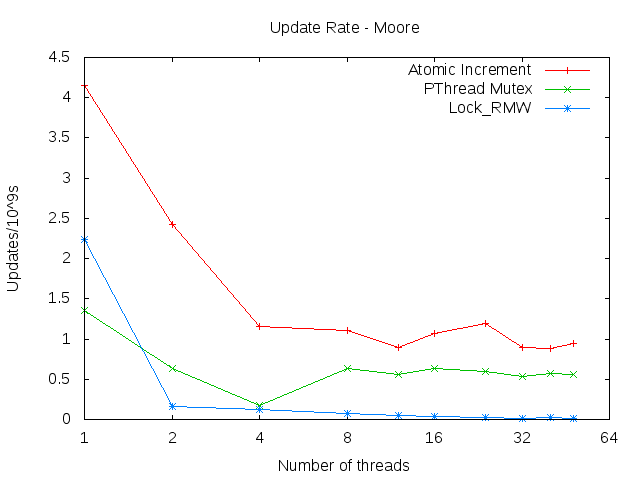
\includegraphics[width=0.7\columnwidth]{Update_rate.png}
\end{center}
As the graphic shows the atomic increment implementation gives the best result. Second is 
the PThread Mutex implementation. We guess that this gap is due to the high overhead for 
the Mutex implementation compared to the simplicity of the atomic operation. The worst 
result is given by our own lock implementation. 
\end{homeworkProblem}

\clearpage
\end{document}
